\documentclass{article}
%\usepackage[utf8]{inputenc}
\usepackage[a4paper, landscape, margin=0.5in]{geometry}
\usepackage{tikz}
\usetikzlibrary{shapes.geometric, arrows,quotes}

\tikzstyle{startstop} = [rectangle, rounded corners, minimum width=2cm, minimum height=1cm,text centered, draw=black, fill=red!30]
\tikzstyle{io} = [trapezium, trapezium left angle=70, trapezium right angle=110, minimum width=2cm, minimum height=1cm, text centered, text width=2cm, draw=black, fill=blue!30]
\tikzstyle{process} = [rectangle, minimum width=2cm, minimum height=1cm, text centered, text width=2cm, draw=black, fill=orange!30]
\tikzstyle{decision} = [diamond, minimum width=1cm, minimum height=1cm, text centered, text width=2cm, draw=black, fill=green!30]
\tikzstyle{arrow} = [thick,->,>=stealth]
\tikzstyle{edge} = [thick,->,>=stealth’,draw,auto]

\begin{document}

\section {plotme level 0 process flow}

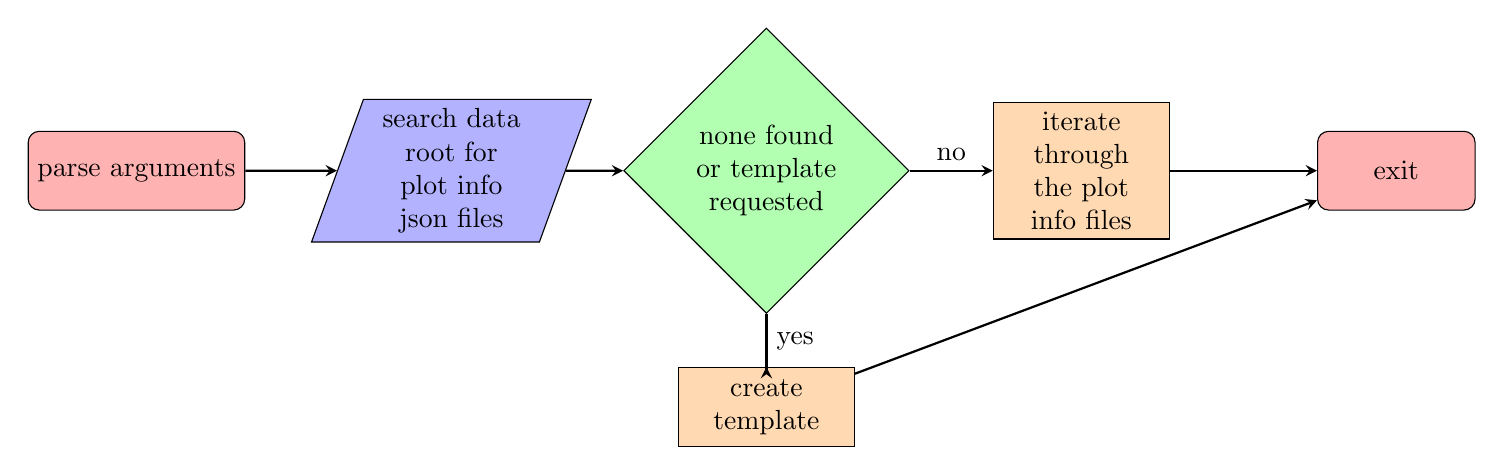
\begin{tikzpicture}[node distance=4cm]
\node (n1) [startstop]{parse arguments};
\node (n2) [io, right of=n1,  xshift=0cm] {search data root for plot info json files};
\node (n3) [decision, right of=n2,  xshift=0cm] {none found or template requested};
\node (n4) [process, below of=n3,  yshift=1cm] {create template};
\node (n5) [process, right of=n3,  xshift=0cm] {iterate through the plot info files};
\node (n6) [startstop, right of=n5, xshift=0cm] {exit};

\draw [arrow] (n1) -- (n2);
\draw [arrow] (n2) -- (n3);
\draw [arrow] (n3.south) to ["yes"] ++  (0, -0.7cm) -| (n4);
\draw [arrow] (n3) -- node[anchor=south] {no} (n5);
\draw [arrow] (n4) -- (n6);
\draw [arrow] (n5) -- (n6);

\end{tikzpicture}

\hspace{1cm}

\section {plotme: Iterate through the plot info files, level 1 process flow}

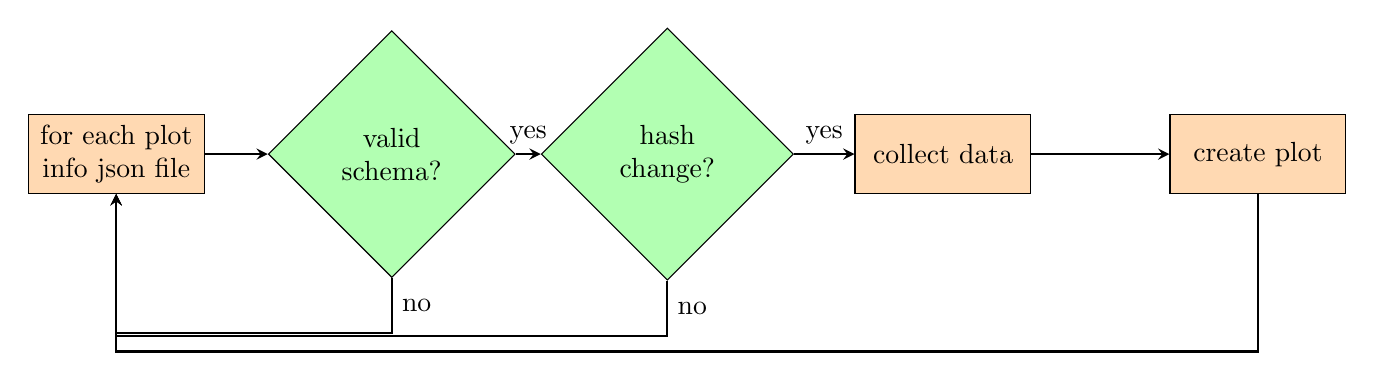
\begin{tikzpicture}[node distance=1.5cm]
\node (n1) [process] {for each plot info json file};
\node (n2) [decision, right of=n1,  xshift=2cm] {valid schema?};
\node (n3) [decision, right of=n2,  xshift=2cm] {hash change?};
\node (n4) [process, right of=n3,  xshift=2cm] {collect data};
\node (n5) [process, right of=n4,  xshift=2.5cm] {create plot};

\draw [arrow] (n1) --  (n2);
\draw [arrow] (n2) -- node[anchor=south] {yes} (n3);
\draw [arrow] (n2.south) to ["no"] ++  (0, -0.7cm) -| (n1);
\draw [arrow] (n3) -- node[anchor=south] {yes} (n4);
\draw [arrow] (n3.south) to ["no"] ++  (0, -0.7cm) -| (n1);
\draw [arrow] (n4) --  (n5);
\draw [arrow] (n5.south) to [""] ++  (0, -2cm) -| (n1);

\end{tikzpicture}
\end{document}